\chapter{Bayesian multi-parameter quantum metrology}
\label{chap:multibayes}

\section{Goals for the final stage of our methodology}

Our study of quantum sensing networks has uncovered a wealth of new results associated with the interplay between correlations and different amounts of data. However, this is only a small part of the rich variety of novel effects that we expect to be relevant for multi-parameter non-asymptotic metrology. While the practical usefulness of our hybrid estimation method (optimal estimator plus asymptotically optimal quantum strategy) will certainly play an important role in exploring this line of thought, it is clear that a limited amount of data demands multi-parameter tools that are specifically designed to take into account the intrinsically Bayesian nature of this type of scenarios.  

In chapter \ref{chap:methodology} we saw that the fundamental equations for the optimal Bayesian quantum strategy have been known since the works of Helstrom, Holevo and others \cite{personick1971, helstrom1976, helstrom1974, holevo1973b, holevo1973, yuen1973}, and in chapter \ref{chap:limited} we exploited this formalism for single-parameter schemes in a way that takes into account the reality of experimental practice, where the resources are always finite and possibly limited. In particular, we have proposed to first calculate the single-shot optimal quantum strategy and then repeat it as many times as the application at hand demands or allows for, and we demonstrated that this procedure generates uncertainties that are optimised in a shot-by-shot fashion and that sometimes recover the Cram\'{e}r-Rao bound asymptotically.

The main task of this chapter is to extend the previous idea to the multi-parameter regime, a goal that will complete the construction of our non-asymptotic methodology. To achieve it, first we will derive a new single-shot lower bound on the multi-parameter uncertainty on the basis of the single-parameter optimum for the square error, so that our result will always be applicable to scenarios where there is a moderate amount of prior information. Then we will discuss how and under which circumstances we can employ our new tool in strategies where the same experiment is repeated several times, and we will illustrate the application of these ideas with two important examples: the two-parameter qubit network that we studied in chapter \ref{chap:networks}, and a discrete model of phase imaging. 

Our findings will provide new insights to understand the role of correlations when we wish to estimate the natural properties (i.e., the original parameters) of some experiment where the data is limited and the prior information is moderate. A comprehensive study of this question was, to the best of our knowledge, missing, since the literature has mainly addressed it using asymptotic tools \cite{proctor2017networked, proctor2017networkedshort, knott2016local, altenburg2018} and the Bayesian part of our analysis in chapter \ref{chap:networks} has been primarily dedicated to the estimation of functions of the original parameters. In addition, we will demonstrate that the multi-parameter Cram\'{e}r-Rao bound is sometimes recovered as a limiting case within our approach. While our results will not be as general as if we could solve the fundamental equations for the multi-parameter optimal strategy in an exact fashion (section \ref{subsec:fundeq}), they will be shown to constitute a reasonable alternative that not only can be applied to real-world problems, but that also relies on calculations that are tractable, both from a numerical and an analytical point of view.

\section{Methodology (part D)}

\subsection{A new multi-parameter single-shot quantum bound}
\label{subsec:mybound}

Suppose we have a probe state $\rho_0$ that is employed to encode the unknown parameters $\boldsymbol{\theta} = (\theta_1, \cdots, \theta_d)$, so that the transformed state is $\rho(\boldsymbol{\theta})$, and that we perform a single measurement $E(m)$ with outcome $m$. Then the likelihood function will be $p(m|\boldsymbol{\theta}) = \mathrm{Tr}[E(m) \rho(\boldsymbol{\theta})]$, and by combining it with the prior $p(\boldsymbol{\theta})$ into the joint density $p(\boldsymbol{\theta}, m) = p(\boldsymbol{\theta}) p(m|\boldsymbol{\theta})$ we can construct the uncertainty
\begin{equation}
\bar{\epsilon}_{\mathrm{mse}} = \sum_{i=1}^d w_i \int d\boldsymbol{\theta} dm ~p(\boldsymbol{\theta}, m) \left[g_i(m) - \theta_i  \right]^2,
\label{msegen}
\end{equation}
where we recall that $g_i(m)$ is the estimator for the $i$-th parameter and $w_i \geqslant 0$ its relative importance. 

In chapter \ref{chap:networks} we saw that the uncertainty in equation (\ref{msegen}) for the parameters $\boldsymbol{\theta}$ arises as a particular case of that in equation (\ref{msefunctions}) for linear functions when we choose the trivial transformation $V = \mathbb{I}$, and provided that we restrict the estimation to a single shot. For that reason, we can now complete the first step of our derivation here, which is to perform a classical optimisation over all the possible estimators, by simply applying the result of such optimisation in section \ref{subsec:multiasymp} for $V = \mathbb{I}$. 

More concretely, let us rewrite equation (\ref{msegen}) as $\bar{\epsilon}_{\mathrm{mse}} = \mathrm{Tr}[\mathcal{W} \Sigma_{\mathrm{mse}}]$, with $\mathcal{W} = \mathrm{diag}(w_1, \dots, w_d)$,
\begin{equation}
\Sigma_{\mathrm{mse}} =  \int d\boldsymbol{\theta} dm ~p(\boldsymbol{\theta}, m) \left[\boldsymbol{g}(m) - \boldsymbol{\theta} \right] \left[\boldsymbol{g}(m) - \boldsymbol{\theta} \right]^\transpose,
\end{equation}
and $\boldsymbol{g}(m) = (g_1(m), \dots, g_d(m))$, and let us recall that, since $\mathcal{W}$ is a positive semi-definite matrix, to minimise $\bar{\epsilon}_{\mathrm{mse}}$ it suffices to lower bound $\Sigma_{\mathrm{mse}}$ in the matrix sense. According to our discussion in section \ref{subsec:multiasymp}, this operation gives us that
\begin{equation}
\Sigma_{\mathrm{mse}} \geqslant \Sigma_{\mathrm{opt}}^c = \int dm~ p(m) \Sigma(m),
\label{optclasmse}
\end{equation}
where $p(m) = \int d\boldsymbol{\theta} p(\boldsymbol{\theta})p(m|\boldsymbol{\theta})$ and
\begin{equation}
\Sigma(m) = \int d\boldsymbol{\theta} p(\boldsymbol{\theta}|m) \boldsymbol{\theta}\boldsymbol{\theta}^\transpose - \left[\int d\boldsymbol{\theta} p(\boldsymbol{\theta}|m) \boldsymbol{\theta}\right] \left[\int d\boldsymbol{\theta} p(\boldsymbol{\theta}|m) \boldsymbol{\theta}\right]^\transpose.
\label{multiexperror}
\end{equation}

Now we observe that by integrating the outcomes in the first term of equation (\ref{multiexperror}), and expanding the posterior  as $p(\boldsymbol{\theta}|m) = p(\boldsymbol{\theta})p(m|\boldsymbol{\theta})/p(m)$ in its second term, we can express $\Sigma_{\mathrm{opt}}^c$ as
\begin{equation}
\Sigma_{\mathrm{opt}}^c = \int d\boldsymbol{\theta} p(\boldsymbol{\theta}) \boldsymbol{\theta}\boldsymbol{\theta}^\transpose - \int \frac{dm}{p(m)}\left[\int d\boldsymbol{\theta} p(\boldsymbol{\theta})p(m|\boldsymbol{\theta}) \boldsymbol{\theta}\right] \left[\int d\boldsymbol{\theta} p(\boldsymbol{\theta})p(m|\boldsymbol{\theta}) \boldsymbol{\theta}\right]^\transpose.
\label{mmsematrix}
\end{equation}
As we can see, the second term of this expression is reminiscent of the definition for the classical Fisher information matrix in equation (\ref{fim}). This is the same type of formal connection between Bayesian quantities and those belonging to the asymptotic theory that we studied in section \ref{subsec:originalderivation} for the single-parameter case, and upon making the quantum part of the problem explicit we can exploit this formal similarity as we did in that section to further lower bound $\Sigma_\mathrm{opt}^c$.

Using equation (\ref{mmsematrix}) and $p(m) = \int d\boldsymbol{\theta} p(\boldsymbol{\theta})p(m|\boldsymbol{\theta})$ we can construct the scalar quantity 
\begin{equation}
\boldsymbol{u}^\transpose \Sigma_{\mathrm{opt}}^c \boldsymbol{u} = \int d\boldsymbol{\theta} p(\boldsymbol{\theta})\theta_u^2 - \int dm  \frac{\left[ \int d\boldsymbol{\theta} p(\boldsymbol{\theta})p(m|\boldsymbol{\theta}) \theta_u \right]^2}{\int d\boldsymbol{\theta} p(\boldsymbol{\theta})p(m|\boldsymbol{\theta})},
\label{scalarquantity}
\end{equation}
where $\theta_u = \boldsymbol{u}^\transpose \boldsymbol{\theta} = \boldsymbol{\theta}^\transpose \boldsymbol{u}$ and $\boldsymbol{u}$ is some real vector, and by inserting $p(m|\boldsymbol{\theta}) = \mathrm{Tr}[E(m) \rho(\boldsymbol{\theta})]$ in equation (\ref{scalarquantity}) we find that
\begin{equation}
\boldsymbol{u}^\transpose \Sigma_{\mathrm{opt}}^c \boldsymbol{u} = \int d\boldsymbol{\theta} p(\boldsymbol{\theta})\theta_u^2 - \int dm  \frac{\mathrm{Tr}\left[ E(m) \bar{\rho}_u \right]^2}{\mathrm{Tr}\left[ E(m) \rho \right]},
\label{bayesanalogy}
\end{equation}
with $\rho = \int d\boldsymbol{\theta} p(\boldsymbol{\theta}) \rho(\boldsymbol{\theta})$ and $\bar{\rho}_u = \int d\boldsymbol{\theta} p(\boldsymbol{\theta}) \rho(\boldsymbol{\theta}) \theta_u$. We have thus arrived at an expression where the second term has taken an analogous form to that of the single-parameter classical Fisher information after having inserted the Born rule, and from our derivation in section \ref{subsec:originalderivation} we know that it is possible to bound this term following the same steps of the proof that gives rise to the Braunstein-Caves inequality for the Fisher information (\cite{BraunsteinCaves1994, genoni2008} and section \ref{subsec:crb}).  

If we follow this analogy and we introduce the Bayesian counterpart of the equation for the symmetric logarithmic derivative, that is, $S_u \rho + \rho S_u = 2\bar{\rho}_u$, then we have that
\begin{align}
\int dm  \frac{\mathrm{Tr}\left[ E(m) \bar{\rho}_u \right]^2}{\mathrm{Tr}\left[ E(m) \rho \right]} &= \int dm\left(\frac{\mathrm{Re}\left\lbrace\mathrm{Tr}\left[E(m) S_u\rho\right]\right\rbrace}{\sqrt{\mathrm{Tr}\left[ E(m) \rho\right]}}\right)^2
\nonumber \\
&\leqslant \int dm~\abs{\frac{\mathrm{Tr}\left[E(m) S_u\rho\right]}{\sqrt{\mathrm{Tr}\left[ E(m) \rho\right]}}}^2
\nonumber \\
&=\int dm~ \abs{\mathrm{Tr}\left[\frac{\rho^{\frac{1}{2}}E(m)^{\frac{1}{2}}}{\sqrt{\mathrm{Tr}\left[ E(m) \rho \right]}} E(m)^{\frac{1}{2}}S_u \rho^{\frac{1}{2}}\right]}^2
\nonumber \\
&\leqslant  \int dm~ \mathrm{Tr}\left[ E(m) S_u \rho S_u \right] = \mathrm{Tr}\left( \rho S_u^2 \right) \equiv \mathcal{K}_u,
\label{quantuminequalities}
\end{align}
where, as in section \ref{subsec:originalderivation}, we have used the Cauchy-Schwarz inequality $|\mathrm{Tr}[X^\dagger Y ]|^2 \leqslant \mathrm{Tr}[ X^\dagger X ] \mathrm{Tr}[Y^\dagger Y ]$ with 
\begin{eqnarray}
X = \frac{E(m)^{\frac{1}{2}} \rho^{\frac{1}{2}}}{\sqrt{\mathrm{Tr}\left[ E(m) \rho \right]}}, ~~Y = E(m)^{\frac{1}{2}} S_u \rho^{\frac{1}{2}}.
\label{csinequality}
\end{eqnarray}

On the other hand, recalling that $\theta_u = \sum_{i=1}^d u_i \theta_i$ we can see that $\bar{\rho}_u = \sum_{i=1}^d u_i \bar{\rho}_i$, with $\bar{\rho}_i = \int d\boldsymbol{\theta} p(\boldsymbol{\theta}) \rho(\boldsymbol{\theta}) \theta_i$. In turn, this allows us to express $S_u$ as $S_u = \sum_{i=1}^d u_i S_i$, with $S_i \rho + \rho S_i = 2\bar{\rho}_i$ and $S_i$ being a Hermitian operator. Since our aim is to derive a matrix inequality, we need to find a way of using the previous definitions to rewrite $\mathcal{K}_u$ as $\mathcal{K}_u = \boldsymbol{u}^\transpose \mathcal{K} \boldsymbol{u}$, where $\mathcal{K}_{ij} = \mathrm{Tr}(\rho A_{ij})$ is a matrix and $A_{ij}$ is some operator associated with the product of $S_i$ and $S_j$. Given that the operators $S_i$ and $S_j$ might not commute, let us first decompose $A_{ij}$ as
\begin{equation}
2 A_{ij} = \left(A_{ij}+A_{ij}^\dagger\right) + \left(A_{ij} - A_{ij}^\dagger\right),
\end{equation}
so that
\begin{equation}
\boldsymbol{u}^\transpose \mathcal{K} \boldsymbol{u} = \frac{1}{2}\left\lbrace\sum_{i, j=1}^d u_i u_j\mathrm{Tr}\left[\rho\left(A_{ij} +  A_{ij}^\dagger\right)\right] + \sum_{i, j=1}^d u_i u_j\mathrm{Tr}\left[\rho\left( A_{ij} - A_{ij}^\dagger\right)\right]\right\rbrace.
\end{equation}
If we were to take $A_{ij} = S_i S_j$, then we would find that 
\begin{align}
\boldsymbol{u}^\transpose \mathcal{K} \boldsymbol{u} &= \frac{1}{2}\left\lbrace\sum_{i, j=1}^d u_i u_j\mathrm{Tr}\left[\rho\left(S_i S_j +  S_j S_i\right)\right] + \sum_{i, j=1}^d u_i u_j\mathrm{Tr}\left[\rho\left( S_i S_j - S_j S_i\right)\right]\right\rbrace
\nonumber \\
&= \frac{1}{2}\left\lbrace\sum_{i, j=1}^d u_i u_j\mathrm{Tr}\left[\rho\left(S_i S_j +  S_j S_i\right)\right] + \mathrm{Tr}\left[\rho\left(S_u^2 - S_u^2\right)\right]\right\rbrace
\nonumber \\
&= \frac{1}{2}\sum_{i, j=1}^d u_i u_j\mathrm{Tr}\left[\rho\left(S_i S_j +  S_j S_i\right)\right] = \mathrm{Tr}\left(\rho S_u^2\right) = \mathcal{K}_u,
\end{align}
and the same result would have been obtained should we had chosen $A_{ij} = S_j S_i$ or the Hermitian version $A_{ij} = (S_i S_j + S_j S_i)/2$ instead. Therefore, we can take $\mathcal{K}$ to be a symmetric matrix with elements\footnote{See \cite{helstrom1968multiparameter} for the analogous operation in the original derivation of the multi-parameter quantum Cram\'{e}r-Rao bound.}
\begin{equation}
\mathcal{K}_{ij} = \mathrm{Tr}\left[\rho \left(S_i S_j + S_j S_i \right) \right]/2.
\label{bayesinfmatrix}
\end{equation}

The combination of equations (\ref{optclasmse}), (\ref{bayesanalogy}), (\ref{quantuminequalities}) and (\ref{bayesinfmatrix}), which must be valid for any $\boldsymbol{u}$, finally gives us the chain of matrix inequalities 
\begin{equation}
\Sigma_{\mathrm{mse}} \geqslant \Sigma_{\mathrm{opt}}^c \geqslant \Sigma_q = \int d\boldsymbol{\theta} p(\boldsymbol{\theta}) \boldsymbol{\theta}\boldsymbol{\theta}^\transpose - \mathcal{K}.
\label{myquantumbound}
\end{equation}
The quantum inequality in equation (\ref{myquantumbound}) is the central result of this chapter.

Applying this result to the original measure of uncertainty in equation (\ref{msegen}) we find that the scalar version of our new bound in equation (\ref{myquantumbound}) is
\begin{equation}
\bar{\epsilon}_\mathrm{mse} \geqslant \sum_{i=1}^d w_i \left[\int d\boldsymbol{\theta} p(\boldsymbol{\theta})\theta_i^2 - \mathrm{Tr}\left(\rho S_i^2\right) \right]. 
\label{multibayesbound}
\end{equation}
Furthermore, by noticing that $\mathrm{Tr}(\rho S_i) = \int d\boldsymbol{\theta} p(\boldsymbol{\theta})\theta_i$ and defining the uncertainties
\begin{equation}
\Delta \theta_{p,i}^2 = \int d\boldsymbol{\theta} p(\boldsymbol{\theta})\theta_i^2 - \left[ \int d\boldsymbol{\theta} p(\boldsymbol{\theta})\theta_i \right]^2
\end{equation}
and $\Delta S_{\rho, i}^2 = \mathrm{Tr}\left(\rho S_i^2 \right) - \mathrm{Tr}\left(\rho S_i \right)^2$ we may rewrite the bound in equation (\ref{multibayesbound}) as
\begin{equation}
\bar{\epsilon}_\mathrm{mse} \geqslant \sum_{i=1}^d w_i \left(\Delta \theta_{p,i}^2 - \Delta S_{\rho, i}^2 \right),
\end{equation}
which is the multi-parameter version of our equivalent expression for a single parameter found in section \ref{subsec:originalderivation}. 

\subsection{Towards a shot-by-shot strategy for many parameters}
\label{subsec:multibayessaturation}

In section \ref{subsec:multiasymp} we saw that the classical inequality in equations (\ref{optclasmse}) and (\ref{myquantumbound}) can be saturated when the estimators are given by the averages over the posterior probability, that is, $\boldsymbol{g}_{\mathrm{opt}}(m) = \int d\boldsymbol{\theta} p(\boldsymbol{\theta}|m)\boldsymbol{\theta}$. On the other hand, since the derivation in equation (\ref{quantuminequalities}) is formally identical to that in section \ref{subsec:originalderivation} for the single-parameter case, from our discussion there we know that the condition for the saturation of the first inequality in equation (\ref{quantuminequalities}) is that $\mathrm{Tr}[E(m)S_u\rho]$ is real, while the second inequality is saturated if and only if
\begin{equation}
\frac{E(m)^{\frac{1}{2}}\rho^{\frac{1}{2}}}{\mathrm{Tr}\left[E(m) \rho \right]} = \frac{E(m)^{\frac{1}{2}}S_u\rho^{\frac{1}{2}}}{\mathrm{Tr}\left[E(m) S_u \rho \right]}.
\end{equation}

If $[S_i, S_j] = 0$ for all $i$, $j$, then we may fulfil such conditions by constructing the measurement scheme with the projections onto the common eigenstates of this set of commuting operators. To verify it, let us first observe that 
\begin{align}
S_u &= \sum_{i=1}^d u_i S_i = \sum_{i=1}^d  u_i \int dm~ c_i(m) \ketbra{\psi(m)} 
\nonumber \\
&= \int dm~c_u(m) \ketbra{\psi(m)},
\end{align}
with $c_u(m) = \sum_{i=1}^d u_i c_i(m)$ and $\lbrace \ketbra{\psi(m)} \rbrace$ being the common eigenstates of $\lbrace S_i \rbrace$. Then, by using $E(m) =  \ketbra{\psi(m)}$ we find that
\begin{align}
\int dm  \frac{\mathrm{Tr}\left[ E(m) \bar{\rho}_u \right]^2}{\mathrm{Tr}\left[ E(m) \rho \right]} &= \int dm\left(\frac{\mathrm{Re}\left\lbrace\mathrm{Tr}\left[\ketbra{\psi(m)} S_u\rho\right]\right\rbrace}{\sqrt{\mathrm{Tr}\left[ \ketbra{\psi(m)} \rho\right]}}\right)^2
\nonumber \\
&= \int dm~ c_u^2(m) \mathrm{Tr}\left[\ketbra{\psi(m)} \rho\right]
\nonumber \\
&= \mathrm{Tr}\left(\rho S_u^2\right) = \mathcal{K}_u = \boldsymbol{u}^\transpose\mathcal{K}\boldsymbol{u},
\end{align}
and, as a consequence, our matrix quantum bound in equation (\ref{myquantumbound}) is achieved. 

The projective strategy based on $\lbrace \ketbra{\psi(m)} \rbrace$ can be thought of as if we were employing the projective measurements that are optimal to estimate each parameter in an independent fashion. Unfortunately, it is known that the optimal strategy for Bayesian multi-parameter estimation is not necessarily based on those projectors \cite{helstrom1974, personick1969thesis}, which is a manifestation of the fact that the quantum estimators $\lbrace S_i \rbrace$ do not need to commute. When $[S_i, S_j] \neq 0$, one possibility would be to search for the projective measurement that is simultaneously optimal for all the parameters. This is precisely what Personick did for $d = 2$ in \cite{personick1969thesis}, where he derived a set of equations for a new set of quantum estimators associated with the simultaneous strategy, and indeed it may be verified that these equations are generally different from those satisfied by $\lbrace S_i \rbrace$. Nevertheless, even if we can find the optimal projective strategy, this might not be optimal in a global sense, since it can be shown \cite{helstrom1974} that to achieve the optimal uncertainty predicted by Helstrom and Holevo's fundamental equations in section \ref{subsec:fundeq} we may need a multi-parameter strategy based on general POMs. In summary, we conclude that we cannot always saturate our bound.  

Despite these difficulties, our new tool can still be useful and informative. On the one hand, the results based on it will be tight and fundamental whenever the operators $\lbrace S_i \rbrace$ commute. If that happens, then the optimal single-shot measurement can be calculated using our bound, and in that case it is possible to generalise our shot-by-shot methodology in chapter \ref{chap:limited} to the multi-parameter regime. In particular, given $\mu$ identical and independent trials and the multi-parameter optimal single-shot POM $\ketbra{\psi(m_i)} \equiv \ketbra{\psi(s_i)}$ with outcome $m_i \equiv s_i$ in the $i$-th repetition, the optimal estimators that take into account the information from all the repetitions of this quantum strategy are $\boldsymbol{g}(\boldsymbol{s}) = \int d\boldsymbol{\theta} p(\boldsymbol{\theta}|\boldsymbol{s}) \boldsymbol{\theta}$, with $\boldsymbol{s} = (s_1, \dots, s_\mu)$, and the associated uncertainty can be expressed as 
\begin{equation}
\bar{\epsilon}_{\mathrm{mse}} = \sum_{i=1}^d w_i \int d\boldsymbol{s}~p(\boldsymbol{s}) \left\lbrace \int d\boldsymbol{\theta} p(\boldsymbol{\theta}|\boldsymbol{s}) \theta_i^2 - \left[\int d\boldsymbol{\theta} p(\boldsymbol{\theta}|\boldsymbol{s}) \theta_i \right]^2 \right\rbrace, 
\label{msegenmany}
\end{equation}
where $p(\boldsymbol{\theta}|\boldsymbol{s}) \propto p(\boldsymbol{\theta}) \prod_{j=1}^\mu \langle \psi(s_j) | \rho(\boldsymbol{\theta}) | \psi(s_j)\rangle$. For $d=2$, which is the case for one of the scenarios that we will study, this error can be numerically calculated as a function of $\mu$ using the two-parameter algorithm presented in section \ref{subsec:multinonasym} and appendix \ref{sec:multimsematlab}.

On the other hand, even if we cannot saturate our bound, it can be argued that it is still better than any other multi-parameter bound for the error in equation (\ref{msegen}) that also ignores the potential non-commutativity of $\lbrace S_i \rbrace$. This is because the latter type of bound will necessarily be equal to or lower than our equation (\ref{multibayesbound}), since the quantity $\int d\boldsymbol{\theta} p(\boldsymbol{\theta})\theta_i^2 - \mathrm{Tr}\left(\rho S_i^2\right)$ is the optimum for the estimation of $\theta_i$ (\cite{personick1971, yuen1973, helstrom1976} and sections \ref{subsec:singleshotparadigm} and \ref{subsec:originalderivation}). The practical consequence of this is that our result will produce bounds that can be tighter than proposals such as the multi-parameter version of the Ziv-Zakai bound in \cite{zhang2014}\footnote{In fact, this has already been demonstrated at the single-parameter level in section \ref{sec:alternativevssingleshot}, where we have found that the Ziv-Zakai and Weiss-Weinstein bounds \cite{tsang2012, tsang2016} are generally loose in optical scenarios with a finite number of repetitions.}. We leave for future work to examine the relative tightness of our bound with respect to other alternatives such as the multi-parameter Weiss-Weinstein bound \cite{tsang2016} or the bound for complex quantities that was derived by Yuen and Lax \cite{yuen1973} when applied to real parameters. 
 
Since the complexity of the calculations associated with our bound is similar to that of the Fisher information matrix for general density operators\footnote{In the single-parameter case this was first observed by Macieszczak \emph{et al.} \cite{macieszczak2014bayesian}.}, with the extra advantage of not having to invert $\mathcal{K}$, we conjecture that the tool that we have introduced may end playing a crucial role in analyses of multi-parameter metrology whenever Helstrom and Holevo's fundamental equations cannot be solved exactly in problems with several parameters. The rest of this chapter is dedicated to demonstrate its usefulness with concrete examples. 

\section{Our methodology in action: results and discussion}

\subsection{Qubit sensing network}
\label{subsec:multibayesqubit}

Our first example is the two-parameter qubit network that we studied in sections \ref{subsec:intersensorasymp} - \ref{subsec:correlationsmultibayes}, which was prepared in the probe state $\ket{\psi_0} = [\ket{00}+\gamma (\ket{01}+\ket{10})+\ket{11}]/\sqrt{2(1+\gamma^2)}$, with real $\gamma$, and which upon interacting with the object that we wish to study was transformed as $\ket{\psi(\theta_1, \theta_2)} = U(\theta_1, \theta_2) \ket{\psi_0}$ by the unitary operator $U(\theta_1, \theta_2) = \mathrm{exp}(-i\sigma_z\theta_1/2)\otimes \mathrm{exp}(-i\sigma_z\theta_1/2) = \mathrm{exp}[-i(\sigma_{z,1}\theta_1 + \sigma_{z,2}\theta_2)/2]$. 

Let us start by performing the single-shot Bayesian analysis. Assuming that we are working in the regime of moderate prior knowledge, so that we can use the flat prior $p(\theta_1, \theta_2) = 4/\pi^2$, when $(\theta_1, \theta_2) \in [-\pi/4, \pi/4]\times[-\pi/4, \pi/4]$, and zero otherwise, we have that\footnote{Unless otherwise indicated, all the analytical calculations of this chapter have been performed using Mathematica.}
\begin{align}
\rho &= \frac{4}{\pi^2}\int_{-\pi/4}^{\pi/4} d\theta_1 \int_{-\pi/4}^{\pi/4} d\theta_2\hspace{0.15em} \mathrm{e}^{-\frac{i}{2}(\sigma_{z,1}\theta_1 + \sigma_{z,2}\theta_2)}\ketbra{\psi_0}\mathrm{e}^{\frac{i}{2}(\sigma_{z,1}\theta_1 + \sigma_{z,2}\theta_2)}
\nonumber \\
&= \frac{1}{2\pi^2(1+\gamma^2)}
\left(
\begin{array}{cccc}
 \pi ^2 & 2 \sqrt{2} \pi  \gamma  & 2 \sqrt{2} \pi  \gamma  & 8 \\
 2 \sqrt{2} \pi  \gamma  & \pi ^2 \gamma ^2 & 8 \gamma ^2 & 2 \sqrt{2} \pi  \gamma  \\
 2 \sqrt{2} \pi  \gamma  & 8 \gamma ^2 & \pi ^2 \gamma ^2 & 2 \sqrt{2} \pi  \gamma  \\
 8 & 2 \sqrt{2} \pi  \gamma  & 2 \sqrt{2} \pi  \gamma  & \pi ^2 \\
\end{array}
\right),
\label{labeleffstate}
\end{align}
\begin{align}
\bar{\rho}_1 &= \frac{4}{\pi^2}\int_{-\pi/4}^{\pi/4} d\theta_1 \int_{-\pi/4}^{\pi/4} d\theta_2\hspace{0.15em} \mathrm{e}^{-\frac{i}{2}(\sigma_{z,1}\theta_1 + \sigma_{z,2}\theta_2)}\ketbra{\psi_0}\mathrm{e}^{\frac{i}{2}(\sigma_{z,1}\theta_1 + \sigma_{z,2}\theta_2)}\theta_1
\nonumber \\
&= \frac{i(4-\pi)}{2\sqrt{2}\pi^2(1+\gamma^2)}
\begin{pmatrix}
0 & 0 & -\pi\gamma & -2\sqrt{2} \\
0 & 0 & -2\sqrt{2}\gamma^2 & -\pi\gamma \\
\pi\gamma & 2\sqrt{2}\gamma^2 & 0 & 0 \\
2\sqrt{2} & \pi\gamma & 0 & 0 
\end{pmatrix},
\label{labeleffmean1}
\end{align}
and
\begin{align}
\bar{\rho}_2 &= \frac{4}{\pi^2}\int_{-\pi/4}^{\pi/4} d\theta_1 \int_{-\pi/4}^{\pi/4} d\theta_2\hspace{0.15em} \mathrm{e}^{-\frac{i}{2}(\sigma_{z,1}\theta_1 + \sigma_{z,2}\theta_2)}\ketbra{\psi_0}\mathrm{e}^{\frac{i}{2}(\sigma_{z,1}\theta_1 + \sigma_{z,2}\theta_2)}\theta_2
\nonumber \\
&= \frac{i(4-\pi)}{2\sqrt{2}\pi^2(1+\gamma^2)}
\begin{pmatrix}
0 & -\pi\gamma & 0 & -2\sqrt{2} \\
\pi\gamma & 0 & 2\sqrt{2}\gamma^2 & 0 \\
0 & -2\sqrt{2}\gamma^2 & 0 & -\pi\gamma \\
2\sqrt{2} & 0 & \pi\gamma & 0 
\end{pmatrix},
\label{labeleffmean2}
\end{align}
where the columns are labelled as $\ket{00}$, $\ket{01}$, $\ket{10}$ and $\ket{11}$. In addition, by inserting equations (\ref{labeleffstate} - \ref{labeleffmean2}) in $S_i\rho + \rho S_i = 2\bar{\rho}_i$, and using a two-parameter extension of the Mathematica algorithm in appendix \ref{sec:singleshotalgorithm}, we find that the independently optimal quantum estimators are
\begin{eqnarray}
S_1 = \frac{2 \left(4-\pi\right)}{\pi\left(1+\gamma^2\right)}\left( \frac{\gamma}{\sqrt{2}} \sigma_y\otimes\mathbb{I} + \frac{1-\gamma^2}{\pi}\sigma_x\otimes\sigma_y \right),
\label{qest1}
\end{eqnarray}
\begin{eqnarray}
S_2 = \frac{2 \left(4-\pi\right)}{\pi\left(1+\gamma^2\right)}\left( \frac{\gamma}{\sqrt{2}} \mathbb{I}\otimes\sigma_y + \frac{1-\gamma^2}{\pi}\sigma_y\otimes\sigma_x \right), 
\label{qest2}
\end{eqnarray}
which have been rewritten in terms of Pauli matrices to better visualise their structure. As a result, the single-shot bound in equation (\ref{multibayesbound}) is
\begin{eqnarray}
\bar{\epsilon}_{\mathrm{mse}} \geqslant \frac{\pi^2}{48} - \frac{2\left(4-\pi\right)^2\left[2-\left(4-\pi^2\right)\gamma^2 + 2\gamma^4 \right]}{\pi^4 \left(1+\gamma^2\right)^2},
\label{qubitoptmse}
\end{eqnarray}
having chosen both parameters to be equally important (i.e., $\mathcal{W} = \mathbb{I}/2$). 

As a first observation we note that equation (\ref{qubitoptmse}) achieves its minimum value at $\gamma = \pm 1$, so that $\bar{\epsilon}_{\mathrm{mse}} \geqslant \pi^2/48 - (4-\pi)^2/(2\pi^2) \approx 0.168$. Given that $\bar{\epsilon}_{\mathrm{prior}} = \pi^2/48 \approx 0.206$, we conclude that a single shot can improve our knowledge about $(\theta_1, \theta_2)$ by $18\%$ with respect to the prior uncertainty\footnote{The improvement is defined as $(\bar{\epsilon}_{\mathrm{prior}}-\bar{\epsilon}_{\mathrm{mse}})/\bar{\epsilon}_{\mathrm{prior}}$ multiplied by $100\%$ (see section \ref{sec:genetic}).}.

\begin{figure}[t]
\centering
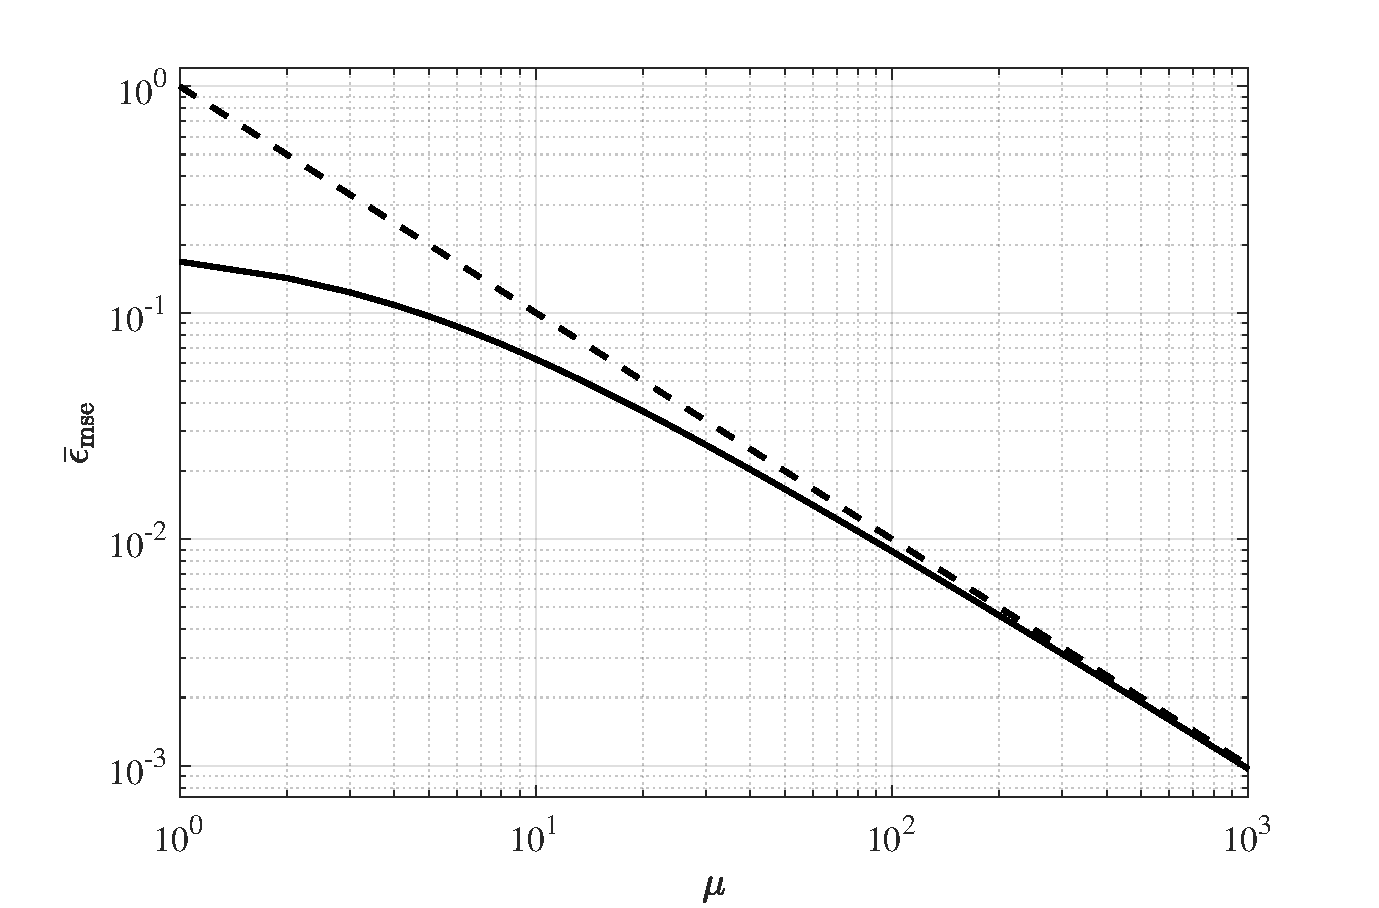
\includegraphics[trim={1cm 0.1cm 1.3cm 1cm},clip,width=14.75cm]{ch7_fig1}
	\caption[Shot-by-shot quantum bound for a two-parameter qubit network]{Mean square error in equation (\ref{msegenmany}) based on a single-shot optimal measurement (solid line) and quantum Cram\'{e}r-Rao bound (dashed line) for the two-parameter qubit network in the main text, with $\gamma = 1$ and a prior squared area $\pi^2/4$ centred around $(0, 0)$. The solid line is the result of optimising the scheme in a shot-by-shot fashion, and it is optimal at least for a single shot and for a large number of them. In addition, note that $\bar{\epsilon}_{\mathrm{cr}} = 1/\mu$ when $\gamma = 1$.}
\label{multibayes_plot}
\end{figure}

Furthermore, since $S_1$ and $S_2$ commute, in this case there is a measurement that achieves our single-shot bound. If we choose $\gamma = 1$, then 
\begin{eqnarray}
S_1 = \frac{ \left(4-\pi\right)}{\pi\sqrt{2}} \sigma_y\otimes\mathbb{I}, ~~S_2 = \frac{ \left(4-\pi\right)}{\pi\sqrt{2}} \mathbb{I}\otimes \sigma_y,
\label{qestloc}
\end{eqnarray}
and thus we can construct an optimal strategy given by the common projectors $\ket{s_+, s_+}$, $\ket{s_-, s_-}$, $\ket{s_+, s_-}$, $\ket{s_-, s_+}$, where $\ket{s_\pm} = (\ket{0}\pm i\ket{1})/\sqrt{2}$. We may then calculate the uncertainty for $\mu$ trials in equation (\ref{msegenmany}) using this measurement in each shot, and the result of this operation has been represented in figure \ref{multibayes_plot} with a solid line. The quantum Cram\'{e}r-Rao bound, which in this case is simply\footnote{To find this result, we first recall that the estimation of the original parameters is equivalent to estimate a set of linear functions with the trivial transformation $V=\mathbb{I}$, for which the geometry parameter is $\mathcal{G} = 0$ (see section \ref{sec:networksasym}), and equation (\ref{crmsetwoqubitnetwork}) indicates that, in this case, the Cram\'{e}r-Rao bound is the expression given in the main text.} $\bar{\epsilon}_{\mathrm{cr}}= \mathrm{Tr}(\mathcal{W} F_q^{-1})/\mu = (1+\gamma^2)^2/(4\mu\gamma^2)$, has also been included in the same figure as the dashed line, and, as we can observe, the latter is approached by the Bayesian error as $\mu$ grows. More concretely, the deviation of the asymptotic bound with respect to the exact calculation reaches the threshold of $\varepsilon_\tau = 0.05$ after $\mu = 5.05 \cdot 10^2$ repetitions (see \ref{subsec:asymsatu} for the definition the relative error $\varepsilon_\tau$), and it further decreases afer that point. Hence, our multi-parameter Bayesian strategy is optimal both for a single shot and for a large number of trials, which is the same behaviour that we found in the single-parameter protocols of chapter \ref{chap:limited}.

Remarkably, our result shows that this scheme does not require entanglement in order to approach the optimal single-shot uncertainty, since the strategy presented above (state plus POM) is local. That a local version of this scheme is optimal to estimate the original parameters was also concluded in \cite{proctor2017networked} from the analysis of its asymptotic performance, and such result may also be recovered from our asymptotic formalism in chapter \ref{chap:networks}. In other words, we have demonstrated that the fact that a global strategy is not needed for this protocol is not only true asymptotically, but also in the non-asymptotic regime when the scheme is implemented in a shot-by-shot fashion with the optimal single-shot measurement.

\subsection{Quantum imaging}

\begin{figure}[t]
\centering
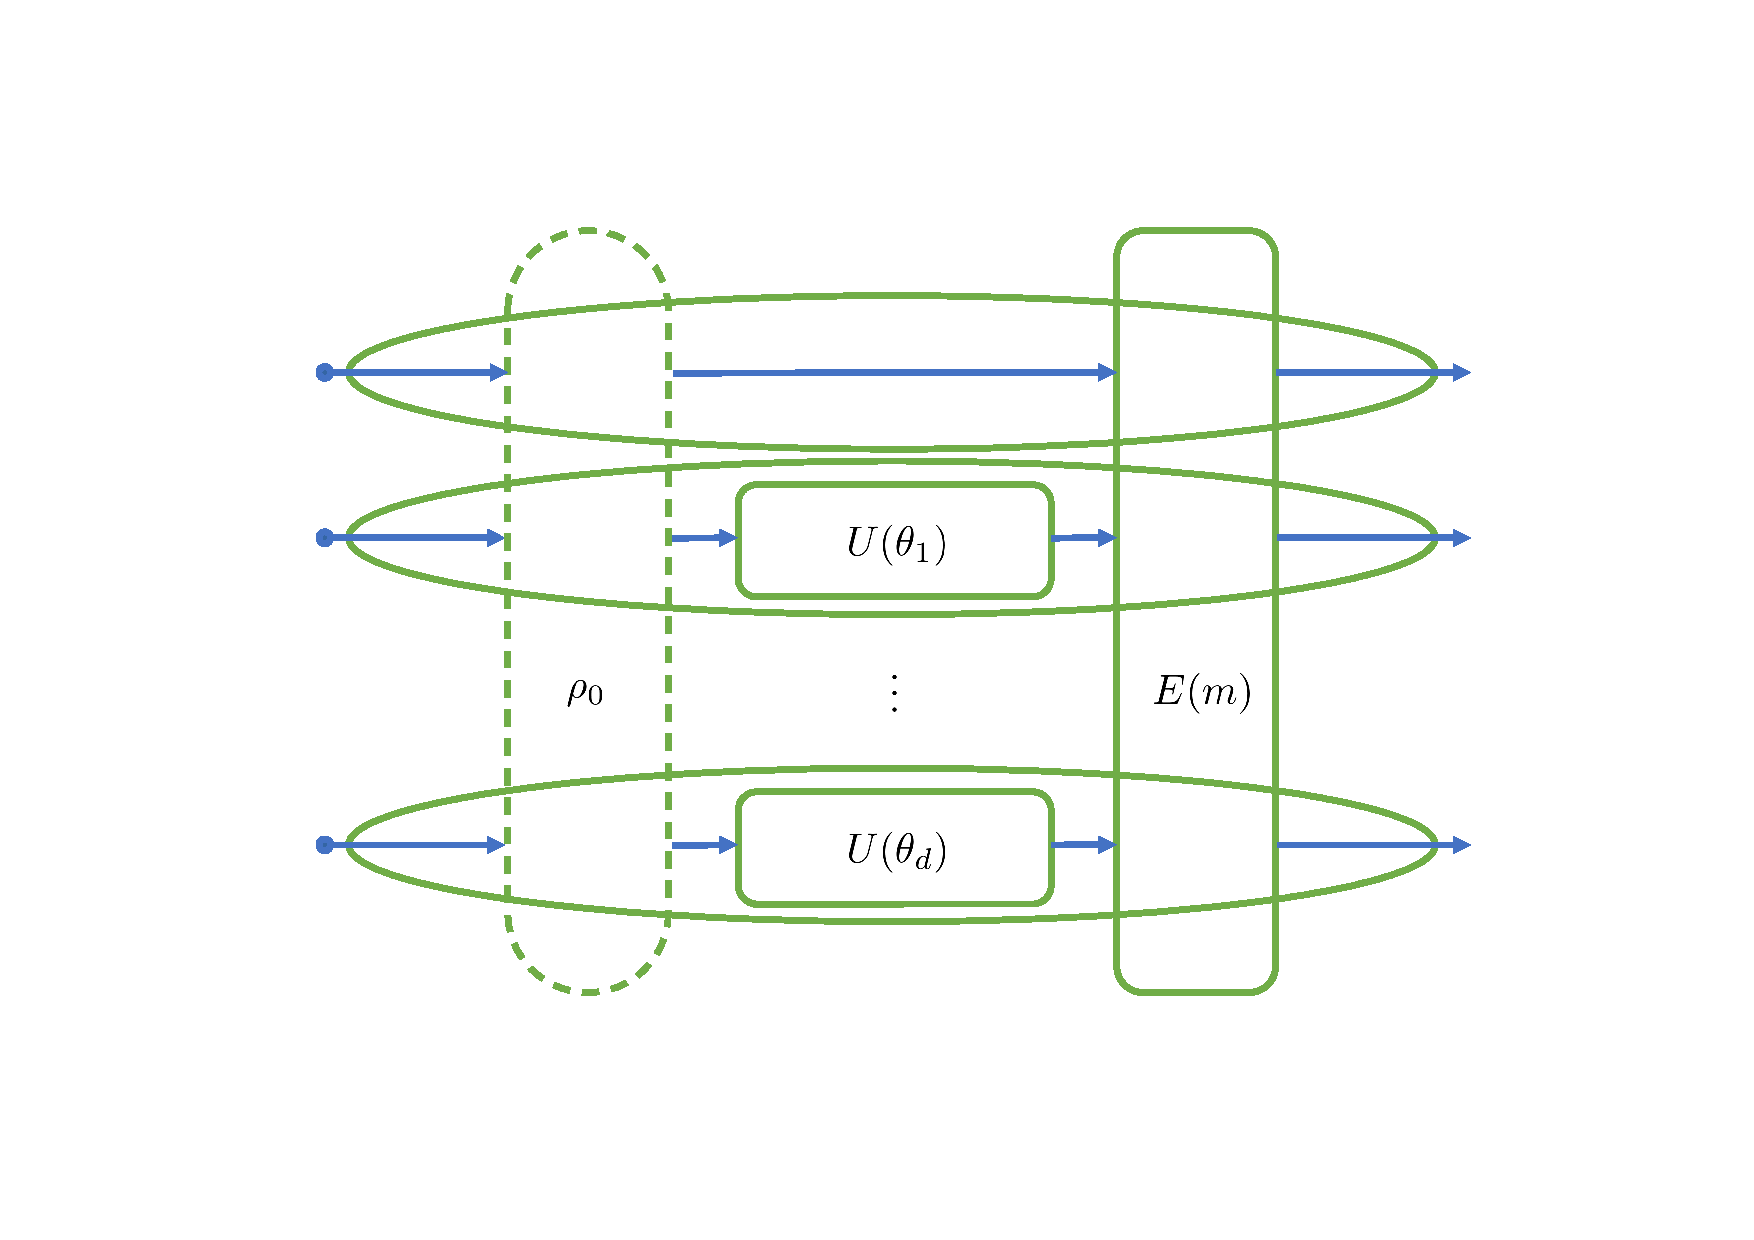
\includegraphics[trim={4.5cm 4cm 4.75cm 3cm},clip,width=12cm]{ch7_fig2}
\caption[Discrete model for phase imaging]{Discrete model for phase imaging, where a collection of $(d+1)$ optical modes are prepared in a (potentially entangled) state $\rho_0$, an unknown parameter $\theta_j$ is encoded in the $j$-th mode via the local unitary operator $U(\theta_j) = \mathrm{exp}(-i a_j^\dagger a_j \theta_j)$ and this operation is repeated for $d$ of them, and a (potentially global) measurement scheme $E(m)$ is implemented, with outcome $m$. As we saw in section \ref{subsec:multischemes}, this scheme is a particular case of the quantum sensing network model proposed by Proctor \emph{et al.} \cite{proctor2017networked} and exploited in chapter \ref{chap:networks}.}
\label{imagingmodel}
\end{figure}

The second scheme that we wish to examine is the discrete model of phase imaging explored by Humphreys \emph{et al.} \cite{humphreys2013} with the Cram\'{e}r-Rao bound, and by Macchiavello \cite{chiara2003} using covariant measurements\footnote{See chapter $4$ of \cite{holevo2011} for an introduction to the concept of \emph{covariant measurement}.}. In the former the scheme is assumed to operate in the asymptotic regime, while in the latter the calculation is carried out for a single shot but in the absence of prior knowledge. On the contrary, our calculations in this section assume an intermediate amount of prior information. 

Consider a system with $(d+1)$ optical modes, such that we encode a phase shift $\theta_j$ with a local unitary $U(\theta_j) = \mathrm{exp}(-i a_j^\dagger a_j \theta_j) = \mathrm{exp}(-i N_j \theta_j)$ in the $j$-th mode, for $1\leqslant j\leqslant d$, while the remaining mode $j=0$ is employed as a reference that has been calibrated in advance \cite{proctor2017networked}. The creation and annihilation operators of the $j$-th mode are $a_j^\dagger$ and $a_j$, respectively, and a schematic representation of this configuration can be found in figure \ref{imagingmodel}. Given this arrangement, a possible strategy is to follow a global approach and prepare the probe as
\begin{equation}
\ket{\psi_0} = \frac{1}{\sqrt{d+\alpha^2}}\left(\alpha\ket{\bar{n}~0 \cdots 0} + \cdots + \ket{0 \cdots 0~\bar{n}} \right),
\label{gnoons}
\end{equation}
which is a generalised NOON state \cite{knott2016local, humphreys2013} with a free parameter $\alpha$ that we take to be real. In this context the resource operator is $R = \sum_{j=0}^{d} N_j$, so that the total amount of resources per trial is given by the mean number of quanta, that is, $\langle \psi_0 |  R | \psi_0 \rangle = \bar{n}$. 

Let us first calculate the single-shot bound on the uncertainty associated with an estimation problem based on this scheme and where $d = 2$, $\bar{n} = 2$, $\mathcal{W} = \mathbb{I}/2$ and the prior probability is the same employed in the qubit case, and let us choose $\alpha = 1$, which is the balanced version of equation (\ref{gnoons}) \cite{knott2016local}. With this configuration we find that 
\begin{eqnarray}
\rho = \frac{1}{3}\left[\mathbb{I} + \frac{2(\lambda_1 + \lambda_4)}{\pi} + \frac{4\lambda_6}{\pi^2} \right],
\end{eqnarray}
and
\begin{eqnarray}
\bar{\rho}_1 = \frac{1}{3\pi}\left(\frac{2\lambda_7}{\pi}-\lambda_2\right),~~\bar{\rho}_2 = -\frac{1}{3\pi}\left(\frac{2\lambda_7}{\pi}+\lambda_5\right),
\end{eqnarray}
where $\lambda_i$ are Gell-Mann matrices\footnote{We recall that the Gell-Mann matrices are defined as \cite{gellmann1962}
\begin{align}
\lambda_1 &=
\begin{pmatrix}
0 & 1 & 0 \\
1 & 0 & 0 \\
0 & 0 & 0
\end{pmatrix},~
\lambda_2 = 
\begin{pmatrix}
0 & -i & 0 \\
i & 0 & 0 \\
0 & 0 & 0
\end{pmatrix},~
\lambda_3 = 
\begin{pmatrix}
1 & 0 & 0 \\
0 & -1 & 0 \\
0 & 0 & 0
\end{pmatrix},~
\lambda_4 =
\begin{pmatrix}
0 & 0 & 1 \\
0 & 0 & 0 \\
1 & 0 & 0
\end{pmatrix},
\nonumber \\
\lambda_5 &= 
\begin{pmatrix}
0 & 0 & -i \\
0 & 0 & 0 \\
i & 0 & 0
\end{pmatrix},~
\lambda_6 = 
\begin{pmatrix}
0 & 0 & 0 \\
0 & 0 & 1 \\
0 & 1 & 0
\end{pmatrix},~
\lambda_7 = 
\begin{pmatrix}
0 & 0 & 0 \\
0 & 0 & -i \\
0 & i & 0
\end{pmatrix},~
\lambda_8 = 
\begin{pmatrix}
1/\sqrt{3} & 0 & 0 \\
0 & 1/\sqrt{3} & 0 \\
0 & 0 & -2/\sqrt{3}
\end{pmatrix}.
\nonumber
\end{align}} \cite{gellmann1962}. Furthermore, introducing these results in $S_k\rho + \rho S_k = 2\bar{\rho}_k$ we find that the quantum estimators are
\begin{equation}
S_1 =  \frac{1}{\pi}\left[ \frac{\lambda_5-(1+\pi^2)\lambda_2}{2+\pi^2}  +\frac{\lambda_7}{\pi} \right],~~S_2 = \frac{1}{\pi}\left[ \frac{\lambda_2 -(1+\pi^2) \lambda_5}{2+\pi^2}  -\frac{\lambda_7}{\pi} \right],
\end{equation}
and the single-shot error is bounded as
\begin{equation}
\bar{\epsilon}_{\mathrm{mse}} \geqslant \frac{\pi^2}{48} - \frac{2\left(4 + 3\pi^2 + \pi^4\right)}{3\pi^4\left(2 + \pi^2\right)} \approx 0.130.
\label{photonbound}
\end{equation}

Unlike in the previous scenario, here $[S_1, S_2] \neq 0$, which implies that the bound does not provide a measurement to apply the shot-by-shot method in an optimal way. However, it can still provide useful information. On the one hand, we can study how close a given measurement can get. A numerical search by trial and error has revealed an approximated set of projectors with a precision almost as good as that given in equation (\ref{photonbound}). In particular, if we use 
\begin{align}
\bra{\varphi_a}&= (0.485 + 0.131 i, 0.441 - 0.070 i, -0.223 + 0.706 i),
\nonumber \\
\bra{\varphi_b} &= (0.688, - 0.208 - 0.432 i, -0.270 - 0.472 i),\nonumber \\
\bra{\varphi_c}&= (0.509 + 0.118 i, -0.284 + 0.700 i, 0.396 )
\end{align}
as the measurement scheme, where the components are labelled as $\ket{2,0,0}$, $\ket{0,2,0}$, $\ket{0,0,2}$, then we have that\footnote{The uncertainty for this POM can be numerically calculated using the MATLAB algorithm in appendix \ref{sec:multimsematlab}.} $\bar{\epsilon}_{\mathrm{mse}} \approx 0.142$. 

On the other hand, we may also explore the precision scaling that the bound is able to predict. In fact, recalling that the scaling associated with the global strategy in equation (\ref{gnoons}) can also be achieved with a local strategy when we work in the asymptotic regime \cite{knott2016local}, it would be desirable to establish whether the same phenomenon can be observed for $\mu = 1$ and a moderate prior.

To study this possibility, suppose we now have $d$ parameters, $\mathcal{W} = \mathbb{I}/d$ and a flat prior of hypervolume $(2\pi/\bar{n})^d$ with $\bar{n} \geqslant 4$, so that the prior knowledge is moderate and sufficient to avoid the periodicities associated with NOON states (see chapters \ref{chap:nonasymptotic} and \ref{chap:limited} and, e.g., \cite{alfredo2017, hall2012, friis2017}). In addition, to simplify the calculation of the bound in equation (\ref{multibayesbound}) let us relabel the components of the state in equation (\ref{gnoons}) as $\beta \equiv 1/\sqrt{d+\alpha^2}$ and $\beta' \equiv \alpha/\sqrt{d+\alpha^2}$, so that $\beta' = \sqrt{1-d\beta^2}$, and the basis kets as
\begin{equation}
\ket{0\dots 0~\bar{n}~0 \dots 0} = \ket{0}_0 \otimes \cdots \otimes \ket{0}_{j-1} \otimes \ket{\bar{n}}_j \otimes \ket{0}_{j+1}\otimes \cdots \ket{0}_d \equiv \ket{u_j}.
\end{equation}
Using these definitions and the fact that
\begin{equation}
\int_{-\frac{\pi}{\bar{n}}}^{\frac{\pi}{\bar{n}}} d\theta_j = \frac{2\pi}{\bar{n}},~~\int_{-\frac{\pi}{\bar{n}}}^{\frac{\pi}{\bar{n}}} d\theta_j \hspace{0.15em} \mathrm{e}^{\pm i \bar{n}\theta_j} \theta_j = \pm \frac{2i \pi}{\bar{n}^2} ,~~\int_{-\frac{\pi}{\bar{n}}}^{\frac{\pi}{\bar{n}}} d\theta_j\hspace{0.15em} \theta_j = \int_{-\pi/\bar{n}}^{\pi/\bar{n}} d\theta_j \hspace{0.15em} \mathrm{e}^{\pm i \bar{n}\theta_j} = 0
\end{equation}
we find that
\begin{align}
\rho &= \left(\frac{\bar{n}}{2\pi}\right)^d \int_{-\frac{\pi}{\bar{n}}}^{\frac{\pi}{\bar{n}}} d\theta_1 \cdots \int_{-\frac{\pi}{\bar{n}}}^{\frac{\pi}{\bar{n}}} d\theta_d \hspace{0.15em}\mathrm{e}^{-i \boldsymbol{N}\cdot\boldsymbol{\theta}} \ketbra{\psi_0}\mathrm{e}^{i \boldsymbol{N}\cdot\boldsymbol{\theta}}
\nonumber \\
&= \left(1 - d\beta^2\right)\ketbra{u_0} + \beta^2 \sum_{k=1}^d \ketbra{u_k},
\label{labeleffstatenoon}
\end{align}
and
\begin{align}
\bar{\rho}_k &= \left(\frac{\bar{n}}{2\pi}\right)^d \int_{-\frac{\pi}{\bar{n}}}^{\frac{\pi}{\bar{n}}} d\theta_1 \cdots \int_{-\frac{\pi}{\bar{n}}}^{\frac{\pi}{\bar{n}}} d\theta_d \hspace{0.15em} \mathrm{e}^{-i \boldsymbol{N}\cdot\boldsymbol{\theta}} \ketbra{\psi_0}\mathrm{e}^{i \boldsymbol{N}\cdot\boldsymbol{\theta}}\theta_k
\nonumber \\
&= \frac{-i\beta \sqrt{1-d\beta^2}}{\bar{n}} \left(\ketbra{u_k}{u_0} - \ketbra{u_0}{u_k}\right).
\end{align}

Next we need to solve $S_k \rho + \rho S_k = 2\bar{\rho_k}$. In section \ref{numcal} we saw that if we decompose $\rho$ as $\rho = \sum_i p_i \ketbra{\phi_i}$, then we can rewrite $S_k$ as
\begin{equation}
S_k = 2 \sum_{i j} \frac{\bra{\phi_i}\bar{\rho_k}\ket{\phi_j}}{p_i + p_j}\ketbra{\phi_i}{\phi_j},
\label{multiqestdiag}
\end{equation}
and by observing that $\rho$ in equation (\ref{labeleffstatenoon}) is already diagonal, equation (\ref{multiqestdiag}) simply becomes
\begin{equation}
S_k =  \frac{- 2i\beta \sqrt{1-d\beta^2}}{\bar{n}\left[1+\beta^2(1-d)\right]} \left(\ketbra{u_k}{u_0} - \ketbra{u_0}{u_k}\right).
\end{equation}

Inserting now the results for $\rho$ and the quantum estimators $S_k$ in equation (\ref{multibayesbound}) we find the bound
\begin{equation}
\bar{\epsilon}_{\mathrm{mse}} \geqslant \frac{1}{\bar{n}^2} \left[\frac{\pi^2}{3} - \frac{4\beta^2 (1-d\beta^2)}{1+\beta^2(1-d)} \right],
\end{equation}
which achieves its minimum at $\beta = 1/\sqrt{d+\sqrt{d}}$ (i.e., at $\alpha = d^{1/4}$). Thus
\begin{equation}
\bar{\epsilon}_{\mathrm{mse}} \geqslant \frac{1}{\bar{n}^2} \left[\frac{\pi^2}{3} - \frac{4}{(1+\sqrt{d})^2} \right] ~\underset{d\gg 1}{\longrightarrow}~ \frac{1}{\bar{n}^2}\left(\frac{\pi^2}{3} - \frac{4}{d}\right)
\label{globalscaling}
\end{equation}
for the global strategy. 

The bound in equation (\ref{globalscaling}) is to be compared to a local protocol such as $\rho_0^{\mathrm{ref}}\otimes \rho_0^{(1)}\otimes \cdots \otimes \rho_0^{(d)}$, with $\rho_0^{(i)} = |\phi_0^{(i)}\rangle \langle \phi_0^{(i)}|$ in the pure case. A choice for $\ket{\phi_0}$ capable of achieving the same asymptotic precision than the generalised NOON state is \cite{knott2016local}
\begin{equation}
\ket{\phi_0} = \left[\sqrt{1- \frac{\bar{n}}{N(d+1)}}\ket{0}+\sqrt{\frac{\bar{n}}{N(d+1)}}\ket{N}\right],
\label{localstrategy}
\end{equation}
where $N$ is a free parameter that can be varied while the total mean number of quanta $\bar{n}$ remains constant. The key idea is that this state can have arbitrarily large local variances as $N$ grows \cite{rivas2012, knott2016local, tsang2012}, so that it belongs to the family of \emph{infinite-precision} states that we examined in section \ref{subsec:infiniteprecision}. As a consequence, if we only used asymptotic tools, then it would appear to be possible not only to equate the performance of the global strategy, but to also supersede this and any other protocol. Nevertheless, the following calculation shows that our Bayesian bound produces a more physical result. 

Given the local strategy in equation (\ref{localstrategy}) and the flat prior of hypervolume $(2\pi/\bar{n})^d$ that we are using, let us express the single-shot bound in equation (\ref{multibayesbound}) as 
\begin{equation}
\bar{\epsilon}_{\mathrm{mse}} \geqslant  \frac{1}{\bar{n}^2} \left[\frac{\pi^2}{3} - f\left(N, \bar{n}, d\right) \right],
\end{equation}
where 
\begin{equation}
f\left(N, \bar{n}, d\right) \equiv \frac{\bar{n}^2}{d} \sum_{k=1}^d \mathrm{Tr}(\rho S_k^2). 
\end{equation}
Since the prior under consideration is separable (that is, $p(\boldsymbol{\theta})=p(\theta_1)\cdots p(\theta_d)$), in this case we have that $\rho = \rho_0^{\mathrm{ref}}\otimes \rho^{(1)}\otimes  \cdots \otimes \rho^{(d)}$ and $\bar{\rho}_k = \rho_0^{\mathrm{ref}}\otimes \rho^{(1)}\otimes  \cdots \otimes \bar{\rho}^{(k)} \otimes  \cdots \otimes \rho^{(d)}$. In turn, the individual quantum estimators take the form $S_k = \mathbb{I}_{\mathrm{ref}}\otimes\mathbb{I}\otimes \cdots \otimes S^{(k)} \otimes\cdots \otimes \mathbb{I}$, and the calculation of the optimal single-shot uncertainty for the local estimation of several phases is effectively reduced to the single-parameter calculation 
\begin{equation}
f\left(N, \bar{n}, d \right) = \bar{n}^2 \hspace{0.15em} \mathrm{Tr}(\varrho S^2),
\label{localfunction}
\end{equation}
where $\rho^{(k)} \equiv \varrho$ and $S^{(k)}\equiv S$ are single-mode operators and $\rho^{(k)}$ and $S^{(k)}$ are identical for all the modes. Performing calculations analogous to those in previous examples (and also similar to those in chapter \ref{chap:limited} for single-parameter NOON states), we find that\footnote{The interested reader can find further details of this calculation in \cite{jesus2019b}.}
\begin{equation}
f\left(N, \bar{n}, d \right) = \frac{4\bar{n}^3\left[\left(1 + d\right) N - \bar{n} \right]\left[N \pi \hspace{0.15em}\mathrm{cos}\left(N\pi/\bar{n}\right) - \bar{n}\hspace{0.15em}\mathrm{sin}\left(N\pi/\bar{n}\right) \right]^2}{\pi^2 N^6 \left(1 + d\right)^2},
\end{equation}
which presents two crucial properties:  
\begin{enumerate}
\item[a)] if $N \rightarrow \infty$, then $f(N,\bar{n},d) \rightarrow 0$, so that
\begin{equation}
\bar{\epsilon}_\mathrm{mse}  ~~\underset{N \rightarrow \infty}{\longrightarrow}~~  \frac{\pi^2}{3 \bar{n}^2} = \frac{1}{d} \sum_{i=1}^d \Delta \theta_{p,i}^2;
\end{equation}
\item[b)] if $N = \bar{n}$, then $f(N,\bar{n},d) = 4d/(1+d)^2$, and
\begin{equation}
\bar{\epsilon}_{\mathrm{mse}} \geqslant \frac{1}{\bar{n}^2}\left[\frac{\pi^2}{3} - \frac{4d}{(1+d)^2}\right] ~~\underset{d\gg 1}{\longrightarrow}~~ \frac{1}{\bar{n}^2}\left(\frac{\pi^2}{3} - \frac{4}{d}\right).
\label{localscaling}
\end{equation}
\end{enumerate}

From the first property it is clear that the local strategy in equation (\ref{localstrategy}) cannot produce an arbitrarily good precision by simply increasing $N$, which contrasts with the performance of these states when one attemps to use the asymptotic theory directly. An intuitive way of understanding this is to observe that the periodicity associated with equation (\ref{localstrategy}) is $2\pi/N$; consequently, the width where the value of a given phase may lie needs to be smaller as $N$ grows to avoid ambiguities, and thus the limit $N \rightarrow \infty$ is essentially equivalent to require that the unknown parameters are practically localised before we perform the estimation. Since the prior knowledge modelled by $p(\boldsymbol{\theta})$ is fixed by the situation under analysis, the high amount of prior information required as $N$ grows is not being provided, and the scheme is eventually unable to extract more information beyond what we knew to start with. This type of behaviour is well understood in single-parameter schemes \cite{tsang2012, berry2012infinite, hall2012, jesus2017, giovannetti2012subheisenberg, pezze2013, rafal2015}, and it complements our discussion about \emph{infinite-precision} states in section \ref{subsec:infiniteprecision}. 

The second property suggests that the global strategy is not required to get the scaling that appears in equations (\ref{globalscaling}) and (\ref{localscaling}), and that this is indeed the case can be shown by verifying that it is possible to reach the bound associated with the local strategy. Recalling that the form of the quantum estimators in the latter case is $S_k =  \mathbb{I}_{\mathrm{ref}}\otimes\mathbb{I}\otimes \cdots \otimes S^{(k)} \otimes\cdots \otimes \mathbb{I}$, we see that this implies that each operator $S_k$ commutes trivially with the rest; consequently, we can always construct an optimal strategy with local states and measurements as we did with the qubit network in section \ref{subsec:multibayesqubit}. This means that the local imaging scheme can be employed to achieve the scaling in equation (\ref{globalscaling}) provided that we choose the prior judiciously and that $N$ is finite, and that a global strategy is not necessary in such case, just as the work in \cite{knott2016local} demonstrated for schemes operating in the asymptotic regime. 

Importantly, note that while we know how to construct a measurement scheme to implement the local strategy for any number of parameters, a strategy whose uncertainty is close to the bound for the global scheme has been found only when $d=2$. We leave for future work to determine whether the scaling in equation (\ref{globalscaling}) can be also recovered by a global protocol such that $\mu = 1$ and $d>2$ and that operates with a moderate amount of prior knowledge.

\section{Summary of results and conclusions}

The method proposed in this chapter provides a framework to study realistic multi-parameter schemes where the empirical data is limited and the prior knowledge is moderate, extending in this way the approach introduced in chapter \ref{chap:limited} for single-parameter scenarios and completing our non-asymptotic methodology for quantum metrology. Taking into account that we are starting to witness the experimental implementation of multi-parameter protocols \cite{roccia2018, polino2018}, our proposal could play a crucial role in the design of future experiments once other realistic effects such as the presence of losses are included.

The application of our method to physical schemes such as a sensing network of qubits or a phase imaging protocol has revealed, in addition, important information about the role of entanglement for the estimation of several parameters, which complements our study of functions of those parameters in chapter \ref{chap:networks}. On the one hand, we have demonstrated that the simultaneous estimation of two parameters using a qubit network can be performed optimally with a local strategy when the number of trials is low and we are working in the intermediate prior information regime. On the other hand, we have seen that the scaling provided by the generalised NOON state can be recovered using a local scheme when $\mu = 1$ and the prior knowledge is moderate. That is, we have shown that the fact that entanglement is not needed to achieve the optimal uncertainty using these schemes is not only true in the asymptotic regime, but also in more realistic configurations. We expect this result to have important consequences in future developments of multi-parameter schemes. 

From a theoretical perspective, the most important result of this chapter is the derivation of a multi-parameter Bayesian bound on the single-shot estimation error. The Bayesian nature of this new tool guarantees that the prior information will be correctly taken into account, and we have demonstrated that our bound can be saturated in some circumstances. Moreover, if that is the case, then we can implement our proposal of performing theoretical metrology analyses by repeating the single-shot optimal strategy, which is one of the central ideas of this thesis.  

To derive our bound we have separated the classical optimisation from the manipulations associated with the quantum part of the problem, as we did in section \ref{subsec:originalderivation} for the single-parameter case. Alternatively, we could have started by constructing the scalar quantity $\boldsymbol{u}^\transpose \Sigma_{\mathrm{mse}}\boldsymbol{u}$, and then we could have instead employed any of the alternative single-parameter proofs available in the literature (see \cite{personick1971, helstrom1976, macieszczak2014bayesian} and our review in section \ref{subsec:singleshotparadigm}) to show that $\boldsymbol{u}^\transpose \Sigma_{\mathrm{mse}}\boldsymbol{u} \geqslant \int d\boldsymbol{\theta}p(\boldsymbol{\theta})\theta_u^2 - \mathrm{Tr}(\rho S_u^2)$, from where equation (\ref{multibayesbound}) follows. Note, however, that in that case the classical and quantum optimisations would be performed simultaneously. 

Among all the bounds that neglect the interference between optimal quantum strategies for different parameters due to their lack of commutativity, our result is arguably the preferred option, since it recovers the true optimum in the limit of a single parameter and gives the true multi-parameter optimum when $\lbrace S_i \rbrace$ commute. Furthermore, our analysis of the qubit network have revealed that the multi-parameter Cram\'{e}r-Rao bound can be recovered as an asymptotic limiting case of our bound, a transition that we have characterised using the method in section \ref{subsec:asymsatu}. Combining these observations with the fact that its calculation is relatively simple, we may conclude that our approach provides a reasonable balance between approaching the exact result and having a tractable problem, and while some care is needed when we use this tool to enquire about fundamental limits, it may be sufficient in many practical cases, as our examples with qubits and optical modes demonstrate. 

The results of this chapter have appeared in \cite{jesus2019b}
\begin{displayquote}
\emph{Bayesian multi-parameter quantum metrology with limited data}, \underline{Jes\'{u}s Rubio} and Jacob Dunningham, arXiv:1906.04123 (2019).
\end{displayquote}